%% ****** Start of file apstemplate.tex ****** %
%%
%%
%%   This file is part of the APS files in the REVTeX 4 distribution.
%%   Version 4.1r of REVTeX, August 2010
%%
%%
%%   Copyright (c) 2001, 2009, 2010 The American Physical Society.
%%
%%   See the REVTeX 4 README file for restrictions and more information.
%%
%
% This is a template for producing manuscripts for use with REVTEX 4.0
% Copy this file to another name and then work on that file.
% That way, you always have this original template file to use.
%
% Group addresses by affiliation; use superscriptaddress for long
% author lists, or if there are many overlapping affiliations.
% For Phys. Rev. appearance, change preprint to twocolumn.
% Choose pra, prb, prc, prd, pre, prl, prstab, prstper, or rmp for journal
%  Add 'draft' option to mark overfull boxes with black boxes
%  Add 'showpacs' option to make PACS codes appear
%  Add 'showkeys' option to make keywords appear
%\documentclass[aps,prl,preprint,groupedaddress]{revtex4-1}
%\documentclass[aps,prl,preprint,superscriptaddress]{revtex4-1}
%\documentclass[aps,prl,reprint,groupedaddress]{revtex4-1}
\documentclass[aps,prd,twocolumn,amsmath,amssymb,amsfont,superscriptaddress]{revtex4-1}
\usepackage{amsmath,aas_macros,xcolor,graphicx}
% You should use BibTeX and apsrev.bst for references
% Choosing a journal automatically selects the correct APS
% BibTeX style file (bst file), so only uncomment the line
% below if necessary.
%\bibliographystyle{apsrev4-1}
\bibliographystyle{h-physrev3}

\newcommand{\bs}{\boldsymbol}
\newcommand{\diff}{{\mathrm d}}
\newcommand{\Cov}{\mathsf{C}}
\newcommand{\Fish}{\mathsf{F}}
\newcommand{\Cl}{\mathcal{C}}
\newcommand{\R}{\mathcal{R}}
\newcommand{\T}{\bold{T}}
\newcommand{\I}{\bold{I}}
\newcommand{\spin}{\bs{j}}
\newcommand{\Msun}{M_\odot}

\newcommand{\tcb}{\textcolor{blue}}
\newcommand{\tcv}{\textcolor{violet}}
\newcommand{\tcr}{\textcolor{red}}
\newcommand{\tcx}{\textcolor{teal}}


\begin{document}

% Use the \preprint command to place your local institutional report
% number in the upper righthand corner of the title page in preprint mode.
% Multiple \preprint commands are allowed.
% Use the 'preprintnumbers' class option to override journal defaults
% to display numbers if necessary
%\preprint{}

%Title of paper
\title{Parity-odd Neutrino Torque Detection}

% repeat the \author .. \affiliation  etc. as needed
% \email, \thanks, \homepage, \altaffiliation all apply to the current
% author. Explanatory text should go in the []'s, actual e-mail
% address or url should go in the {}'s for \email and \homepage.
% Please use the appropriate macro foreach each type of information

% \affiliation command applies to all authors since the last
% \affiliation command. The \affiliation command should follow the
% other information
% \affiliation can be followed by \email, \homepage, \thanks as well.
\author{Hao-Ran~Yu}\email{\url{haoran@cita.utoronto.ca}}
\affiliation{Tsung-Dao Lee Institute, Shanghai Jiao Tong University, Shanghai, 200240, China}
\affiliation{Canadian Institute for Theoretical Astrophysics, University of Toronto, M5S 3H8, Ontario, Canada}
\affiliation{Department of Astronomy, Shanghai Jiao Tong University, Shanghai, 200240, China}

\author{Ue-Li~Pen}\email{\url{pen@cita.utoronto.ca}}
\affiliation{Canadian Institute for Theoretical Astrophysics, University of Toronto, M5S 3H8, Ontario, Canada}
\affiliation{Tsung-Dao Lee Institute, Shanghai Jiao Tong University, Shanghai, 200240, China}
\affiliation{Dunlap Institute for Astronomy and Astrophysics, University of Toronto, Toronto, ON M5S 3H4, Canada}
\affiliation{Canadian Institute for Advanced Research, CIFAR Program in Gravitation and Cosmology, Toronto, ON M5G 1Z8, Canada}
\affiliation{Perimeter Institute for Theoretical Physics, Waterloo, ON N2L 2Y5, Canada}

\author{Xin~Wang}\email{\url{xwang@cita.utoronto.ca}}
\affiliation{Canadian Institute for Theoretical Astrophysics, University of Toronto, M5S 3H8, Ontario, Canada}

%Collaboration name if desired (requires use of superscriptaddress
%option in \documentclass). \noaffiliation is required (may also be
%used with the \author command).
%\collaboration can be followed by \email, \homepage, \thanks as well.
%\collaboration{}
%\noaffiliation

\date{\today}

\begin{abstract}
Cosmological observations are promising ways to improve of our understandings of the neutrino mass properties. 
The upper bound on their sum of mass is given by the cosmic microwave background and large scale structures. 
These measurements are all parity-even. 
Here we show that, the presence of neutrino mass provides a unique contribution to the directions of the angular momentum  of galaxies, which is the first parity-odd neutrino effect on large scale structures. 
This parity-odd observable is free of the contamination of the linear perturbation theory, and can be cleanly separated from other non-gravitational effects. 
A complete 21-cm neutral Hydrogen halo survey deep to redshift 1 can give a $5\sigma$ confidence level of detecting the neutrino torque effect if the sum of neutrino masses is 0.05 eV.

\end{abstract}

% insert suggested PACS numbers in braces on next line
\pacs{}
% insert suggested keywords - APS authors don't need to do this
%\keywords{}

%\maketitle must follow title, authors, abstract, \pacs, and \keywords
\maketitle

\tcb{\textit{Introduction.---}}
Neutrino mass is a long-standing physics problem. 
The flavour oscillation experiments \citep{2002PhRvL..89a1301A} discovered the mass 
splittings of neutrinos and placed a lower bound of the sum of their mass 
$M_\nu \equiv \sum_{i=1}^3 m_{\nu_i} \gtrsim$ 0.05 eV \citep{2014ChPhC..38i0001O}. 
The existence of neutrino mass has profound impacts on cosmic evolution. 
In the early Universe relativistic neutrinos modulate the matter-to-radiation ratio, 
and based on which the cosmic microwave background observations provide an 
upper bound of $M_\nu\lesssim 0.23$ eV \citep{2016A&A...594A..13P}. 
In the late Universe, neutrinos become non-relativistic, 
and contribute to the matter energy density $\Omega_m$. 
Unlike the majority of matter, the cold dark matter (CDM) and baryons, 
neutrinos maintain a high velocity dispersion, 
known as ``free streaming'', which reduces their gravitational collapse on small scales. 
A number of large scale structure (LSS) surveys 
(such as Euclid \cite{2011arXiv1110.3193L},
LSST \cite{2009arXiv0912.0201L}, eBOSS \cite{2016AJ....151...44D}, WFIRST\cite{2012SPIE.8442E..1UG}, 
and DESI \cite{2015AAS...22533605E}) are aimed to improve this upper bound using neutrino effects on LSS, 
however we usually encounter difficulties in disentangling neutrino effects from other parameters, 
and in understanding halo bias and cosmic variance. 
Recently, new nonlinear neutrinos effects on LSS are proposed to give independent measurements on neutrino mass \citep{2014PhRvL.113m1301Z,2016PhRvL.116n1301Z,2017NatAs...1E.143Y}. 
For these effects one needs to carefully separate and exclude the contaminations from non-gravitational contributions. 
The only clean, gravitational-only neutrino effect on LSS is the damping of weak gravitational lensing power spectrum \citep{2016A&A...594A..13P}. 
However the amount of information and constraining power of the lensing is limited by the projection onto the 2-dimensional sky. 
Is there a 3-dimensional measure which is cleanly gravity-driven, to measure the neutrino mass?

The angular momentum. The angular momenta (spin) of dark matter halos or galaxies originated by clean gravitational interactions. 
Unlike parity-even tidal and density fields, the linear perturbation theory (other effects and bias) cannot contaminate a parity-odd spin measurement. 
Here we present the neutrino torque effect, to modulate the spin of dark matter halos.

\tcb{\textit{Theory.---}} 
In the picture of LSS formation, gravitational instability lets initial density fluctuations form dark matter halos, in which galaxies are embedded.
In these highly nonlinear structures, uncertainties of halo bias, 
halo merging history and baryonic mechanisms obstruct us from clearly 
understanding the statistics like number counts and morphologies.
In comparison, the spins of galaxies/halos represent a local probe of gravity, 
especially contributed from the linear epoch of the structure formation. 

In the tidal torque theory, the spin of a halo in Lagrangian space $\spin_L\propto\int_{V_L}\bs{q}\times\bs{\nabla}\phi\diff^3\bs{q}$ 
can be written in first order as $\spin_I\propto\bs{\epsilon}\,\I\,\T$ \citep{1984ApJ...286...38W}, 
where $\phi$ is the gravitational potential, $\bs{q}$ is the Lagrangian coordinates relative to the center of mass of the protohalo in volume $V_L$, 
$\I_q=(I_{ij})=(\int_{V_L} q_i q_j \diff^3\bs{q})$ is the protogalactic inertia tensor, 
$\T=(T_{ij})=(\partial_i\partial_j\phi)$ is the local tidal shear tensor, 
and $\bs{\epsilon}=(\epsilon_{ijk})$ is the Levi-Civita symbol to collect the asymmetric components generated by
the misalignment between $\I_q$ and $\T$. This spin grows at first order in the early Universe \citep{1984ApJ...286...38W}. 
Actually, as halos collapse, nonlinear gravity field is hard to torque small objects, and the spin directions are expected  to be contributed mostly in the linear regime. These concepts can be straightforwardly tested in numerical simulations. 
In Lagrangian space, CDM and baryonic matter are torqued by the same gravitational shear, so the spin direction is not affected by baryonic effects. 
If a halo has a merging history, it simply collects disconnected regions in Lagrangian space but conserves their total spin. 

Massive neutrinos contribute sub-percent fraction of the matter ingredient, and their unique spatial distribution and evolution should contribute a unique torque to halos and galaxies.
In particular, neutrino density field traces CDM on large scales while their small scale structures are smoothed out by their high velocity dispersion, known as the free-streaming. 
They contribute a predictable tidal tensor $\T_\nu(m_{\nu_i})$ depending on the their mass. 
The interplay between $\I_q$ and $\T_\nu$ leads to an additional neutrino torque $\spin^I_\nu\propto\bs{\epsilon}\,\I_q\,\T_\nu$.
Integrated neutrino torque over cosmic evolution, we get the neutrino modulation of the halo spin,
\begin{equation}\label{eq.jnu0}
\spin^I_{\nu 0}=\int a(\tau)D(\tau)\bs{\epsilon}\I(\tau)\T_\nu(\tau)\diff\tau.
\end{equation}
Here, $\tau$ is the Newtonian time, $D(\tau)$ is the growth factor, and other quantities are functions of time.

\tcb{\textit{Reconstruction.---}} 
The feasibility of prediction of the neutrino tidal torque relies on the precision reconstruction of the cosmic evolution history. 
There are many emerging reconstruction methods. 
For example, the isobaric halo reconstruction can recover the initial conditions of the universe from spatial distribution of halos. 
In the case of high number densities the reconstructed density field is correlated with the true initial density field on scales $k\lesssim 0.7 h/{\rm Mpc}$ \citep{2017ApJ...847..110Y}, 
close to the limit ($k\lesssim 1 h/{\rm Mpc}$) of isobaric reconstruction from using direct CDM density field \citep{2017PhRvD..96l3502Z}, 
or the limit of reconstruction from the true displacement field \citep{2017PhRvD..95d3501Y}. 
ELUCID simulation are able to reconstruct the local Universe \citep{2014ApJ...794...94W}.
These reconstruction techniques enable us to study the tidal field from both CDM and neutrinos in an unprecedented precision, at different epochs of the cosmic evolution. 
Neutrinos share the same Fourier phases of CDM, reconstructed from halo reconstruction, but only differ by the ratio of their linear transfer function, depending on the neutrino masses.
The final neutrino torque can be understood as the interaction between large (neutrino free streaming) and small (collapsing) scales.

To apply Eq.(\ref{eq.jnu0}), $\I_q$ is also required to be reconstructed. 
Firstly, we note the fact that, during the initial conditions, the $\I_q$ and $\T_c$ are highly correlated in Lagrangian space \citep{2000ApJ...532L...5L,2001ApJ...555..106L}, 
which can be understood that $\I_q$ is a collection of matter to be shell-crossed to form a halo, being parallel with $\T_c$.
Secondly, in the linear, intermediate epochs, $\I_q$ is firstly reshaped according to the dominating $\T_c$, thus the linear evolved $\T_\nu(\tau)$ will act on an evolved $\I(\tau)$.
Further, $\I(\tau)$ will be affected by nonlinear effects, which are more difficult to predict, however halos are relatively small and their spin directions can hardly be changed dramatically.
\tcb{A deeply study of the second step above is beyond the scope of this letter. Here we show that, even simplified to the first point above, the total neutrino torque can still be reconstructed.}

We construct an equivalent inertia $\I_r$ from $\T_c$, in order that $\bs{\epsilon}\,\I_r\T_\nu$ is maximumly correlated with $\spin^I_{\nu 0}$ from Eq.(\ref{eq.jnu0}).
In the primary coordinate of $\T_c$, $\T_c$ can be eigen-decomposed as $\T_c=\sum_{i=1}^3\T^{\lambda_i}_c$ and find $\alpha_i$ such that the reconstructed
\begin{equation}\label{eq.Ir}
	\I_r=\sum_{i=1}^3\alpha_i\T^{\lambda_i}_c
\end{equation}
optimizes the cross-correlation $\mu(\spin^I_{\nu 0},\spin^{I_r})$, where
\begin{equation}\label{eq.jnuIr}
 	\spin^{I_r}_\nu=\bs{\epsilon}\,\I_r\T_\nu
\end{equation}
is the reconstructed neutrino spin direction.


\begin{figure}
\centering
  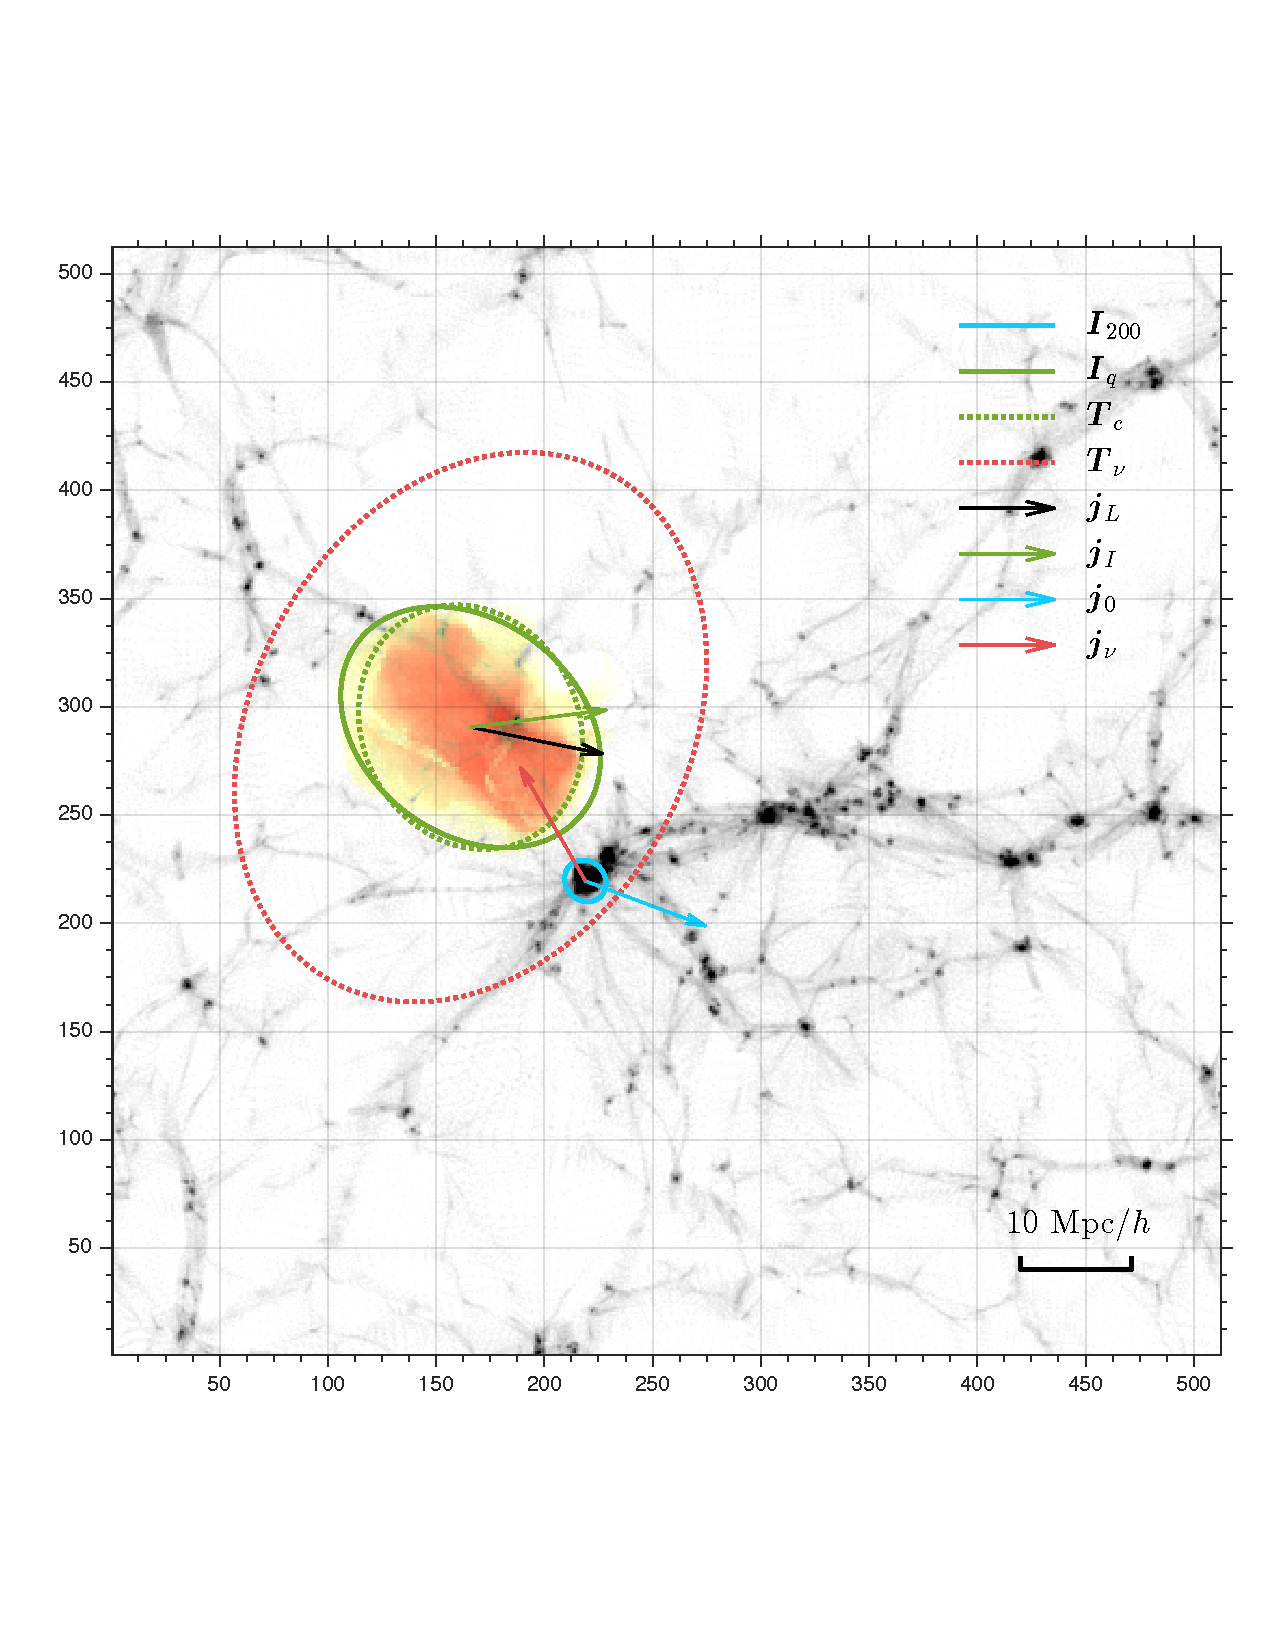
\includegraphics[width=1\linewidth]{f1}
 \caption{Visualization of the neutrino torque. 
 We show the LSS slice centered at a selected halo with depth twice the halo radius $r_{200}$. 
 Equivalent ellipsoids by solid lines show the moment of inertia in Lagrangian and Eulerian space $\I_q$ and $\I_{200}$, 
 while dotted ellipsoids show the tidal shear from CDM and neutrinos $\T_c$ and $\T_\nu$. $\spin_L$, 
 $\spin_0$ are the Lagrangian and Eulerian halo spins, whereas $\spin_I$ is the tidal torque prediction. 
 The initial neutrino torque is shown by $\spin_\nu$.}\label{fig.1}
\end{figure}
\tcb{\textit{Simulation.---}}
These correlations and coefficients are tested across a set of high-resolution $N$-body simulations \citep{2018ApJS..237...24Y}. 
Given any halo formed in the simulation, all the belonging particles are mapped back to Lagrangian space. 
The status of this definite set of particles can be traced in a resimulation of the exact same initial conditions.

In Fig.\ref{fig.1} (all quantities are projected onto the plane of this letter), 
we select a very massive halo ($7.8\times 10^{14}M_\odot$) to maximize the clarity of the visualization of the halo properties.
Note that these properties (cross-correlations) have only weak dependence on halo mass. 
The background LSS at redshift $z=0$ has the thickness $2r_{200}$ with $r_{200}$ being the halo radius within which the mean halo density is 200 times the mean matter density of the Universe.
The Lagrangian mapping of this halo is shown by the protohalo's column density with the orange clouds.
To visualize the tidal torque theory, we plot ellipsoids equivalent to $\I_q$ and 
$\I_{200}$, where $\I_{200}$ is the moment of inertia within $r_{200}$. 
The ellipsoids with dotted lines correspond to $\T_c$ and $\T_\nu$, normalized such that their volumes are $V_L$ and $8V_L$ respectively. 
As expected, $\I_q$ and $\T_c$ are aligned with their primary axes in parallel with the collapsing direction, or perpendicular to the filament below. 
Their minor misalignment yields the tidal torque $\spin_I$ (all the spin arrows are normalized to have 15 Mpc$/h$), which is the first order approximation of the true initial spin $\spin_L$. 
They are, in general, highly correlated with the spin of the final halo $\spin_0$.
In comparison, the neutrino tidal shear $\T_\nu$ torques $\I_q$ in an other less correlated direction $\spin_\nu$.

The validity of the tidal torque formulation is tested by an ensemble average over all halos, 
across 3 orders of magnitude in mass range, and over simulations with different resolutions.
the cross-correlation coefficients $\left\langle \spin(z) \cdot \spin_L \right\rangle$ and
$\left\langle \spin(z) \cdot \spin_I \right\rangle$ smoothly decrease from 1 to 0.80, and
from 0.75 to 0.69, respectively.

For neutrinos, the first-order tidal torque approximation gives a perfect (with cross-correlation 0.99) representation of the actual neutrino torque and it has generally less than 0.2 cross-correlation with CDM torques. This is expected in that $\T_c$ dominates locally \tcr{(power spectrum index?)} whereas $\T_\nu$ is contributed beyond the neutrino free-streaming scale \tcr{(is this a 4-point function?)}. These two species, however, have a highly correlated contribution in structure formation. When we consider the forces that the two species exerted to the protohalo, $\bs{F}_{c/\nu}\propto\int_{V_L}\bs{\nabla}\phi_{c/\nu}\diff^3\bs{q}$, the cross-correlation between two species is as high as 0.86 \tcr{(power spectrum index?)}.

By Eq.(\ref{eq.jnu0}) we estimate the magnitude of integrated neutrino torque $\left\langle|\spin_{0\nu}|/|\spin_0|\right\rangle\simeq 3\times10^{-4}$. In particular, the effect given by the smoother distribution for neutrinos relative to CDM accounts 0.03, while the neutrino fraction $f_\nu=3.5\times 10^{-3}$ (for $M_\nu=0.05$ eV) and the backreaction from neutrinos to CDM \tcr{$\sqrt{8}$} contribute the rest.

Measured from simulations, $(\alpha_1,\alpha_2,\alpha_3)=(-0.18,0.18,0.02)$ in Eq.(\ref{eq.Ir}) optimizes the cross-correlation $\left\langle\spin^I_{\nu 0}\cdot\spin^{I_r}_\nu\right\rangle=0.19$. In this case we need $5\times 10^9$ halos to have a $5\sigma$ detection (see Appendix A). If we improve the reconstruction of $\I_R$, the lower limit of required halos is $2\times 10^8$. 

\tcb{\textit{Discussion.---}} 
Accuracy and mass dependency: we notice that the cross-correlation coefficients between $\spin_0$ and initial values $\spin_L$ and $\spin_T$ are prominently higher than what was measured in \citep{2000ApJ...532L...5L}. We investigate that numerical errors that may affect the results. P3M (particle-particle particle-mesh) algorithms result in higher cross-correlation between initial and final spins, compared to PM (particle-mesh), where additional tangential forces in PM violate the angular momentum conservation. Higher mass halos in a given simulation generally have slightly higher $\mu_L$ and $\mu_I$, however the correlation is enhanced greatly as we use higher mass resolutions. All other cross-correlation measurements have only weak dependencies on the halo mass, even in a fixed simulation. With different box sizes, mass resolutions, force resolutions, and find that the results are consistent across these simulations. Especially, in the estimation of number of halo spins needed to detect the neutrino torque, the deciding number is the cross-correlation $\left\langle\spin^I_{\nu 0}\cdot\spin^{I_r}_\nu\right\rangle=0.19$. This has a very weak dependence on halo mass and configuration of the simulation.

Baryonic effects (+ etc.) in reconstruction and angular momentum conservation:

Observability: surveys like the Hubble Sphere Hydrogen Survey (HSHS) \citep{2006astro.ph..6104P} can cover 1 billion galaxies. There are xxx HI galaxies with redshift 1 \citep{2004MNRAS.350.1210Z}.

Beyond standard models: it was also suggested that neutrino mass is generated by a gravitational $\theta$-term condensation as the source of dark energy \citep{2016PhRvD..93k3002D}.

Cosmic variance:

Bias:

cite later \citep{2018MNRAS.tmp.2447C}.

\tcb{\textit{Conclusion.---}} 

\tcb{\textit{Acknowledgments.---}}
We acknowledge funding from NSERC.

% body of paper here - Use proper section commands
% References should be done using the \cite, \ref, and \label commands
%\section{}
% Put \label in argument of \section for cross-referencing
%\section{\label{}}
%\subsection{}
%\subsubsection{}

% If in two-column mode, this environment will change to single-column
% format so that long equations can be displayed. Use
% sparingly.
%\begin{widetext}
% put long equation here
%\end{widetext}

% figures should be put into the text as floats.
% Use the graphics or graphicx packages (distributed with LaTeX2e)
% and the \includegraphics macro defined in those packages.
% See the LaTeX Graphics Companion by Michel Goosens, Sebastian Rahtz,
% and Frank Mittelbach for instance.
%
% Here is an example of the general form of a figure:
% Fill in the caption in the braces of the \caption{} command. Put the label
% that you will use with \ref{} command in the braces of the \label{} command.
% Use the figure* environment if the figure should span across the
% entire page. There is no need to do explicit centering.

% \begin{figure}
% \includegraphics{}%
% \caption{\label{}}
% \end{figure}

% Surround figure environment with turnpage environment for landscape
% figure
% \begin{turnpage}
% \begin{figure}
% \includegraphics{}%
% \caption{\label{}}
% \end{figure}
% \end{turnpage}

% tables should appear as floats within the text
%
% Here is an example of the general form of a table:
% Fill in the caption in the braces of the \caption{} command. Put the label
% that you will use with \ref{} command in the braces of the \label{} command.
% Insert the column specifiers (l, r, c, d, etc.) in the empty braces of the
% \begin{tabular}{} command.
% The ruledtabular enviroment adds doubled rules to table and sets a
% reasonable default table settings.
% Use the table* environment to get a full-width table in two-column
% Add \usepackage{longtable} and the longtable (or longtable*}
% environment for nicely formatted long tables. Or use the the [H]
% placement option to break a long table (with less control than 
% in longtable).
% \begin{table}%[H] add [H] placement to break table across pages
% \caption{\label{}}
% \begin{ruledtabular}
% \begin{tabular}{}
% Lines of table here ending with \\
% \end{tabular}
% \end{ruledtabular}
% \end{table}

% Surround table environment with turnpage environment for landscape
% table
% \begin{turnpage}
% \begin{table}
% \caption{\label{}}
% \begin{ruledtabular}
% \begin{tabular}{}
% \end{tabular}
% \end{ruledtabular}
% \end{table}
% \end{turnpage}

% Specify following sections are appendices. Use \appendix* if there
% only one appendix.
\appendix
\section{Errors in 3D}
There are $N$ halos with their unit spin vector randomly distributed on a 2D sphere, $|\spin|=1$ and $\left\langle \spin \right\rangle =\bs{0}$. Adding an additional vector $a\hat{\bs{x}}$ ($a\ll 1$) to $\spin$ and normalize we have $\spin'=(\spin+a\hat{\bs{x}})/|\spin+a\hat{\bs{x}}|$, then we project $\spin'$ onto $\hat{\bs{x}}$ and we get the signal $b=\spin'\cdot\hat{\bs{x}}$. The numerical statistics are as following: $\left\langle b \right\rangle=2a/3$ and $\sigma(b)=1/\sqrt{3N}$. So, to get a $n\sigma$ detection, 
\begin{equation}
	N=3n^2/4a^2 
\end{equation}
halos will be needed.

% If you have acknowledgments, this puts in the proper section head.
%\begin{acknowledgments}
% put your acknowledgments here.
%\end{acknowledgments}

% Create the reference section using BibTeX:
\bibliography{haoran_ref}

\end{document}
%
% ****** End of file apstemplate.tex ******

